\documentclass{config/apuntes}

\title{Bioinformática Estructural}
\author{Sandra Mingo Ramírez}
\date{2024/25}
\acronym{STRBIO}

\usepackage[all]{nowidow}
\usepackage{listing}
\usepackage{color}
\usepackage{tabularx}
\usepackage{multirow}
\usepackage{makecell}
\usepackage{amsmath}
\usepackage{array}
\usepackage{soul}

\definecolor{dkgreen}{rgb}{0,0.6,0}
\definecolor{gray}{rgb}{0.5,0.5,0.5}
\definecolor{mauve}{rgb}{0.58,0,0.82}

\lstset{
  frame=tb,
  aboveskip=3mm,
  belowskip=3mm,
  showstringspaces=false,
  columns=flexible,
  basicstyle={\small\ttfamily},
  numbers=none,
  numberstyle=\tiny\color{gray},
  keywordstyle=\color{blue},
  commentstyle=\color{dkgreen},
  stringstyle=\color{mauve},
  breaklines=true,
  breakatwhitespace=true,
  tabsize=3
}

\usepackage{tocloft}

\advance\cftchapnumwidth 0.9em\relax
\advance\cftsecnumwidth 0.6em\relax
\advance\cftsubsecindent 0.5em\relax
\advance\cftsubsecnumwidth 0.5em\relax
\begin{document}

\begin{abstract}
La biología estructural permite el estudio de las estructuras de macromoléculas, el origen de esta estructura y su relación con la función biológica. La función específica está íntimamente ligada a la conformación tridimensional; la configuración estructural de las biomoléculas depende a su vez de su composición básica. Por ello, se busca obtener y comprender diferentes resultados de modelado de estructuras proteicas para resolver problemas biológicos. También es importante comprender las bases teóricas, tanto conceptuales como algorítmicas, de la predicción y análisis de estructura de macromoléculas, e interpretar los resultados de estos programas.
\end{abstract}

\pagestyle{plain}

\maketitle

\tableofcontents

%Tema 1: Aplicaciones y métodos de bioinformática estructural en biología y biomedicina
%Tema 2: Aplicaciones para visualización de estructuras 3D de moléculas biológicas
%Tema 3: Métodos alternativos para la predicción de estructuras secundarias y terciarias de proteínas
%Tema 4: Acoplamiento (docking) computacional de proteínas y fármacos
%Examen 40% 
%Prácticas 60%
	%5% play with secondary structures and protein DDBB
	%15% working with structures
	%30% casp-like exercise
	%5% randomized peer-assessment -> opcional, es un 5% adicional en la asignatura
	%10% docking
	%Electronic Lab Notebook: esto es el objetivo, esto es lo que hemos hecho, esto es lo que hemos conseguido

%29/01 - Modesto
\part{Introducción y modelado de proteínas}
\chapter{Aplicaciones y métodos de bioinformática estructural en biología y biomedicina}
\section{Metas en la bioinformática estructural}
La bioinformática estructural (SB por sus siglas en inglés) es una disciplina amplia que abarca recursos de datos, algoritmos y herramientas para investigar, analizar, predecir e interpretar estructuras biomacromoleculares. En este curso, nos centraremos específicamente en la bioinformática estructural de proteínas, incluyendo la visualización y el análisis de la estructura de biomacromoléculas, así como la predicción de estructuras y complejos de proteínas. La premisa de la SB es que la información estructural de alta resolución sobre los sistemas biológicos permite un razonamiento preciso sobre sus funciones y los efectos de las modificaciones y perturbaciones.

Los objetivos de SB requieren al menos cuatro líneas de investigación diferentes:
\begin{itemize}
\item \textbf{Visualización}: Tratar con una o muchas estructuras complejas e integrar varias fuentes de información como secuencias, datos estructurales, campos electrostáticos, localizaciones de sitios funcionales y áreas de variabilidad.
\item \textbf{Clasificación}: Agrupación jerárquica de estructuras similares para identificar orígenes comunes y vías de diversificación. Al igual que en otros campos de la biología, la clasificación es tediosa pero necesaria para comprender el espacio estructural.
\item La \textbf{predicción} de estructuras sigue siendo un área de gran interés y un campo de investigación en sí mismo. Como veremos a continuación, el número de secuencias diferentes es mucho mayor que la disponibilidad de estructuras, lo que hace de la predicción una herramienta esencial y útil.
\item \textbf{Simulación}: Las estructuras obtenidas experimentalmente son ante todo modelos estructurales estáticos. Sin embargo, las propiedades de estas moléculas son a menudo el resultado de sus movimientos dinámicos. La definición de las funciones energéticas que rigen el plegamiento de las proteínas y su posterior dinámica estable pueden analizarse mediante simulaciones de dinámica molecular, aunque las capacidades de cálculo pueden ser limitantes para alcanzar escalas de tiempo biológicamente relevantes.
\end{itemize}

Impulsado por enormes cantidades de datos e importantes avances técnicos, este campo ha experimentado una transformación sustancial en los últimos veinte años. La mejora de las capacidades experimentales para analizar la estructura de las proteínas y otras moléculas y estructuras biológicas y el avance de la predicción de estructuras asistida por Inteligencia Artificial (IA) han aumentado sustancialmente la capacidad de los investigadores de las ciencias de la vida para abordar diversas cuestiones relativas a la diversidad, evolución y función de las proteínas. Esta transformación se ha potenciado en los últimos 5 años, y sus implicaciones para la biología, la biotecnología y la biomedicina siguen siendo en gran medida impredecibles.

\section{Introducción a las estructuras proteicas}
Las proteínas son componentes esenciales de la vida, que intervienen en diversas funciones vitales como elementos estructurales, elementos de andamiaje o enzimas activas que catalizan reacciones metabólicas. Las proteínas están compuestas por polímeros de aminoácidos, y la secuencia de aminoácidos de una proteína concreta se denomina \textbf{estructura primaria} de la proteína. Las cadenas de aminoácidos pueden plegarse espontáneamente en estructuras tridimensionales, estabilizadas principalmente por enlaces de hidrógeno entre aminoácidos. La secuencia de aminoácidos determina las diferentes capas de la estructura tridimensional. En la naturaleza existen L-aminoácidos, pero no D-aminoácidos. Cada uno de los 20 aminoácidos naturales tiene propiedades fisicoquímicas específicas que influyen en su conformación preferida. Por lo tanto, el nivel inicial de plegamiento se conoce como \textbf{estructura secundaria}, que forma patrones comunes como se verá más adelante. Estos segmentos de patrones de estructura secundaria son capaces de plegarse en formas tridimensionales debido a las interacciones entre las cadenas laterales de los aminoácidos, lo que se conoce como \textbf{estructura terciaria} de la proteína. Además, dos o más cadenas peptídicas individuales pueden agregarse para formar proteínas multisubunidad, lo que se conoce como \textbf{estructura cuaternaria}.

\begin{figure}[h]
\centering
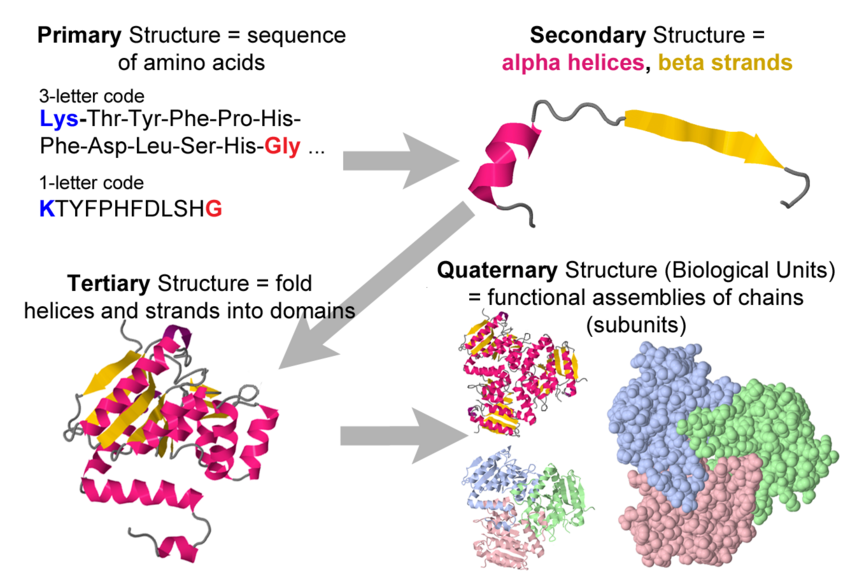
\includegraphics[width = 0.6\textwidth]{figs/850px-Protein-structure-4-levels-III-flat.png}
\caption{Los distintos niveles de la estructura proteica.}
\end{figure}

Es importante señalar que el enlace peptídico en sí no permite la rotación, ya que posee características parciales de doble enlace. Por lo tanto, la rotación está restringida a los enlaces entre el C$\alpha$ y el grupo C = O (el ángulo phi ($\phi$)) y el C$\alpha$ y el grupo NH (el ángulo psi ($\psi$)). Así pues, la cadena principal del polipéptido consiste en una secuencia repetida de dos enlaces giratorios seguidos de un enlace no giratorio (péptido). Sin embargo, no todos los 360º de los ángulos $\phi$ y $\psi$ son factibles debido a posibles \textbf{choques estéricos} entre cadenas laterales vecinas. Para determinados ángulos y combinaciones de aminoácidos, las restricciones espaciales impiden que los átomos ocupen la misma ubicación física, lo que explica en parte las distintas propensiones de ciertos aminoácidos a adoptar diferentes tipos de estructuras secundarias. 

\begin{figure}[h]
\centering
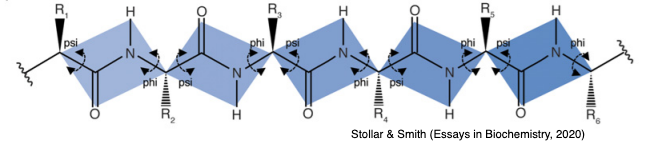
\includegraphics[width = 0.8\textwidth]{figs/peptide_bond.png}
\caption{Esquema de una cadena polipeptídica genérica. Las cadenas laterales de los residuos se denotan como R. Los rectángulos coloreados indican conjuntos de seis átomos que son coplanares debido al carácter de doble enlace del enlace peptídico. Las flechas indican los enlaces que son libres de rotar con el ángulo de rotación sobre el N-C$\alpha$ conocido como phi ($|phi$) y sobre el C$\alpha$-C conocido como psi ($\psi$). Obsérvese que sólo se etiquetan los enlaces del esqueleto peptídico y que, en la mayoría de los casos, el enlace del grupo R es libre de rotar.}
\end{figure}

Además, las cadenas laterales de los aminoácidos poseen sus propios ángulos de torsión, conocidos como $\chi1$, $\chi2$, $\chi3$, etc (figura \ref{fig:chi}). Estos ángulos de torsión influyen significativamente en las estructuras secundarias y, sobre todo, terciarias de las proteínas. Las distintas combinaciones de torsiones de las cadenas laterales definidas por los ángulos $\chi$ se denominan \textbf{rotámeros}.

\begin{figure}[h]
\centering
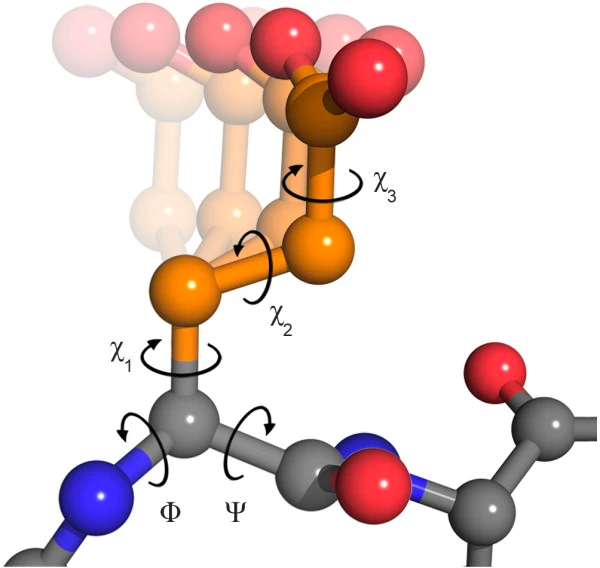
\includegraphics[width = 0.3\textwidth]{figs/paste-6EE800AE.png}
\caption{Ángulos diedros en el glutamato: Los ángulos diedros son los principales grados de libertad de la columna vertebral (ángulos $\phi$ y $\psi$) y la cadena lateral (ángulos $\chi$) de un aminoácido. El número de ángulos $\chi$ varía entre cero y cuatro para los 20 aminoácidos estándar. La figura muestra una representación esférica del glutamato, que tiene tres $\chi$ ángulos.}
\label{fig:chi}
\end{figure}

Dentro de estas limitaciones, las dos conformaciones locales primarias que evitan el impedimento estérico y maximizan el enlace de hidrógeno entre la columna vertebral y el backbone son las estructuras secundarias $\alpha$-hélice y $\beta$-hoja. Linus Pauling propuso inicialmente la hélice $\alpha$ como zurda en 1951, pero la estructura cristalina de la mioglobina en 1958 reveló que la forma diestra es más común. En las hélices diestras típicas, el grupo NH de la espina dorsal se une mediante enlaces de hidrógeno al grupo C=O de la espina dorsal del aminoácido situado cuatro residuos antes en la secuencia de la proteína. Esta forma de espiral regular tiene los grupos R apuntando hacia fuera, lejos de la espina dorsal peptídica, y requiere unos 3,6 residuos para completar una vuelta completa de la hélice (figura \ref{fig:alfa}).

\begin{figure}[h]
\centering
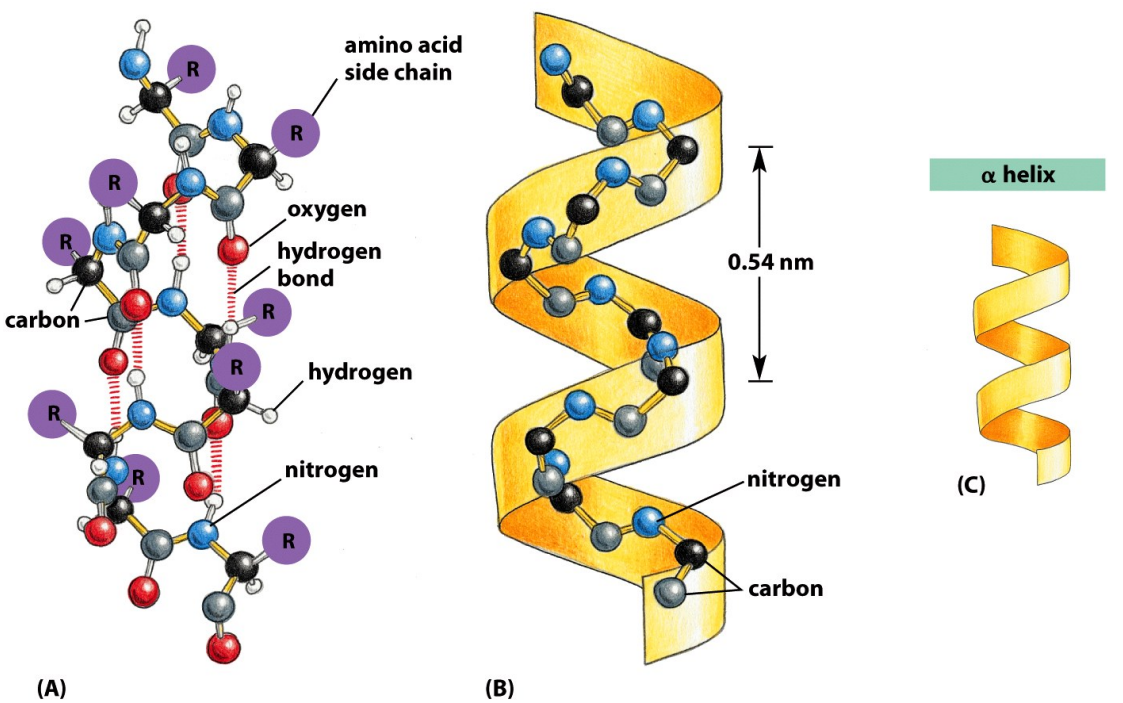
\includegraphics[width = 0.6\textwidth]{figs/alpha.png}
\caption{Hélice alfa.}
\label{fig:alfa}
\end{figure}

Las diferentes secuencias de aminoácidos tienen distintas tendencias a formar estructuras $\alpha$-helicoidales. La metionina, la alanina, la leucina, el glutamato y la lisina tienen propensiones especialmente altas a formar hélices, mientras que la prolina y la glicina tienen propensiones pobres a formar hélices. La prolina a menudo rompe o retuerce una hélice porque carece de un hidrógeno amida para formar enlaces de hidrógeno y su voluminosa cadena lateral interfiere con el esqueleto del giro precedente. La glicina, con sólo un hidrógeno como grupo R, es demasiado flexible y costosa desde el punto de vista entrópico para mantener la estructura $\alpha$-helicoidal, lo que la convierte en una rompedora de hélices $\alpha$.

\begin{figure}[h]
\centering
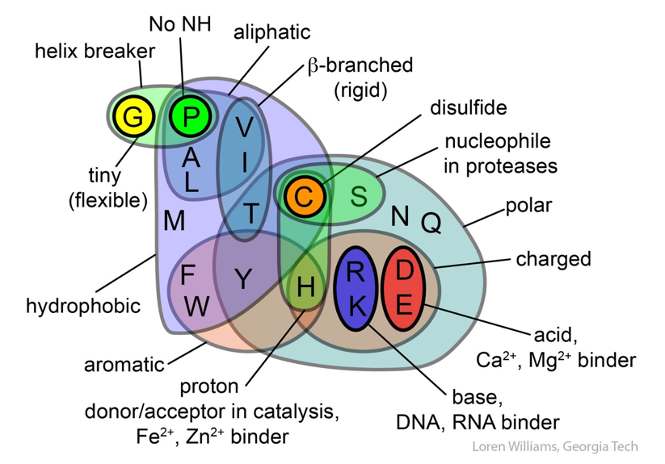
\includegraphics[width = 0.5\textwidth]{figs/aa.png}
\caption{Aminoácidos clasificados según su tipo.}
\end{figure}

Las láminas $\beta$ (figura \ref{fig:beta}) están formadas por dos o más cadenas polipeptídicas extendidas denominadas hebras $\beta$ que discurren una junto a otra en disposición paralela o antiparalela. En una lámina $\beta$, los residuos se disponen en zigzag y los enlaces peptídicos adyacentes apuntan en direcciones opuestas. El grupo NH y el grupo C=O de cada aminoácido forman enlaces de hidrógeno con el grupo C=O y el grupo NH, respectivamente, de las cadenas adyacentes. Las cadenas pueden ir en direcciones opuestas (lámina $\beta$ antiparalela) o en la misma dirección (lámina $\beta$ paralela). Las cadenas laterales de cada residuo se alternan en direcciones opuestas, dando a las láminas $\beta$ caras hidrofílicas e hidrofóbicas, formando a menudo un patrón de alternancia de residuos hidrofílicos e hidrofóbicos en la estructura primaria.

\begin{figure}[h]
\centering
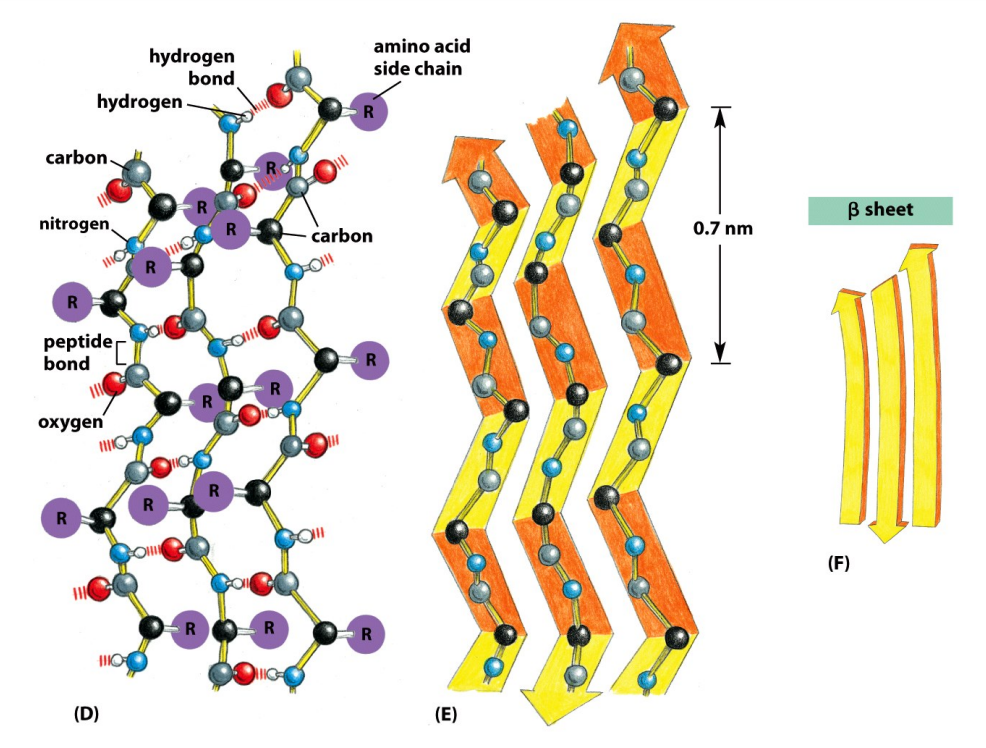
\includegraphics[width = 0.6\textwidth]{figs/beta.png}
\caption{Descripción detallada de una lámina beta formada por tres hebras beta.}
\label{fig:beta}
\end{figure}

Los residuos aromáticos grandes (tirosina, fenilalanina, triptófano) y los aminoácidos $\beta$-ramificados (treonina, valina, isoleucina) suelen encontrarse en las hebras $\beta$. Como en el caso de las hélices $\alpha$, las hebras $\beta$ suelen estar terminadas por glicinas, que son especialmente comunes en los giros $\beta$ (el conector más común entre hebras), como aminoácidos con ángulos $\phi$ positivos.

Las estructuras secundarias, terciarias y cuaternarias de las proteínas se mantienen gracias a las interacciones entre aminoácidos (figura \ref{fig:interactions}). Estas interacciones suelen clasificarse en cuatro tipos, que pueden ser tanto intra- como intermoleculares:
\begin{enumerate}
\item \textbf{Enlace iónico}: Los enlaces iónicos surgen de las atracciones electrostáticas entre cadenas laterales de aminoácidos cargadas positiva y negativamente. Por ejemplo, la atracción entre un ion carboxilato del ácido aspártico y un ion amonio de la lisina ayuda a estabilizar una región plegada específica de una proteína.
\item \textbf{Enlace de hidrógeno}: Los enlaces de hidrógeno se forman entre un átomo de oxígeno o nitrógeno altamente electronegativo y un átomo de hidrógeno unido a otro átomo de oxígeno o nitrógeno, como los de las cadenas laterales de aminoácidos polares. Los enlaces de hidrógeno son cruciales para las interacciones intra e intermoleculares en las proteínas, como en las hélices alfa.
\item \textbf{Enlaces disulfuro}. Cuando dos aminoácidos cisteína se acercan durante el plegamiento de la proteína en condiciones redox adecuadas, la oxidación puede unir sus átomos de azufre, formando un enlace disulfuro. A diferencia de los enlaces iónicos o de hidrógeno, se trata de enlaces covalentes, por lo que son un ejemplo clásico de reacción espontánea, que se produce como modificación postraduccional. Aunque son sensibles a los agentes reductores, estabilizan en gran medida la estructura terciaria y son vitales para la estructura cuaternaria de muchas proteínas, como los anticuerpos.
\item \textbf{Interacciones hidrofóbicas}. Las fuerzas de dispersión surgen cuando un átomo normalmente no polar se convierte momentáneamente en polar debido a una distribución desigual de electrones, dando lugar a un dipolo instantáneo que induce un desplazamiento de electrones en un átomo no polar vecino. Las fuerzas de dispersión son débiles, pero pueden ser importantes cuando otros tipos de interacciones no existen o son mínimas. El término interacción hidrofóbica suele utilizarse erróneamente como sinónimo de fuerzas de dispersión. Las interacciones hidrofóbicas surgen porque las moléculas de agua establecen enlaces de hidrógeno con otras moléculas de agua (o grupos de proteínas capaces de establecer enlaces de hidrógeno). Como los grupos no polares no pueden formar enlaces de hidrógeno, la proteína se pliega de tal forma que estos grupos quedan enterrados en la parte interior de la estructura proteica, minimizando su contacto con el agua.
\end{enumerate}

\begin{figure}[h]
\centering
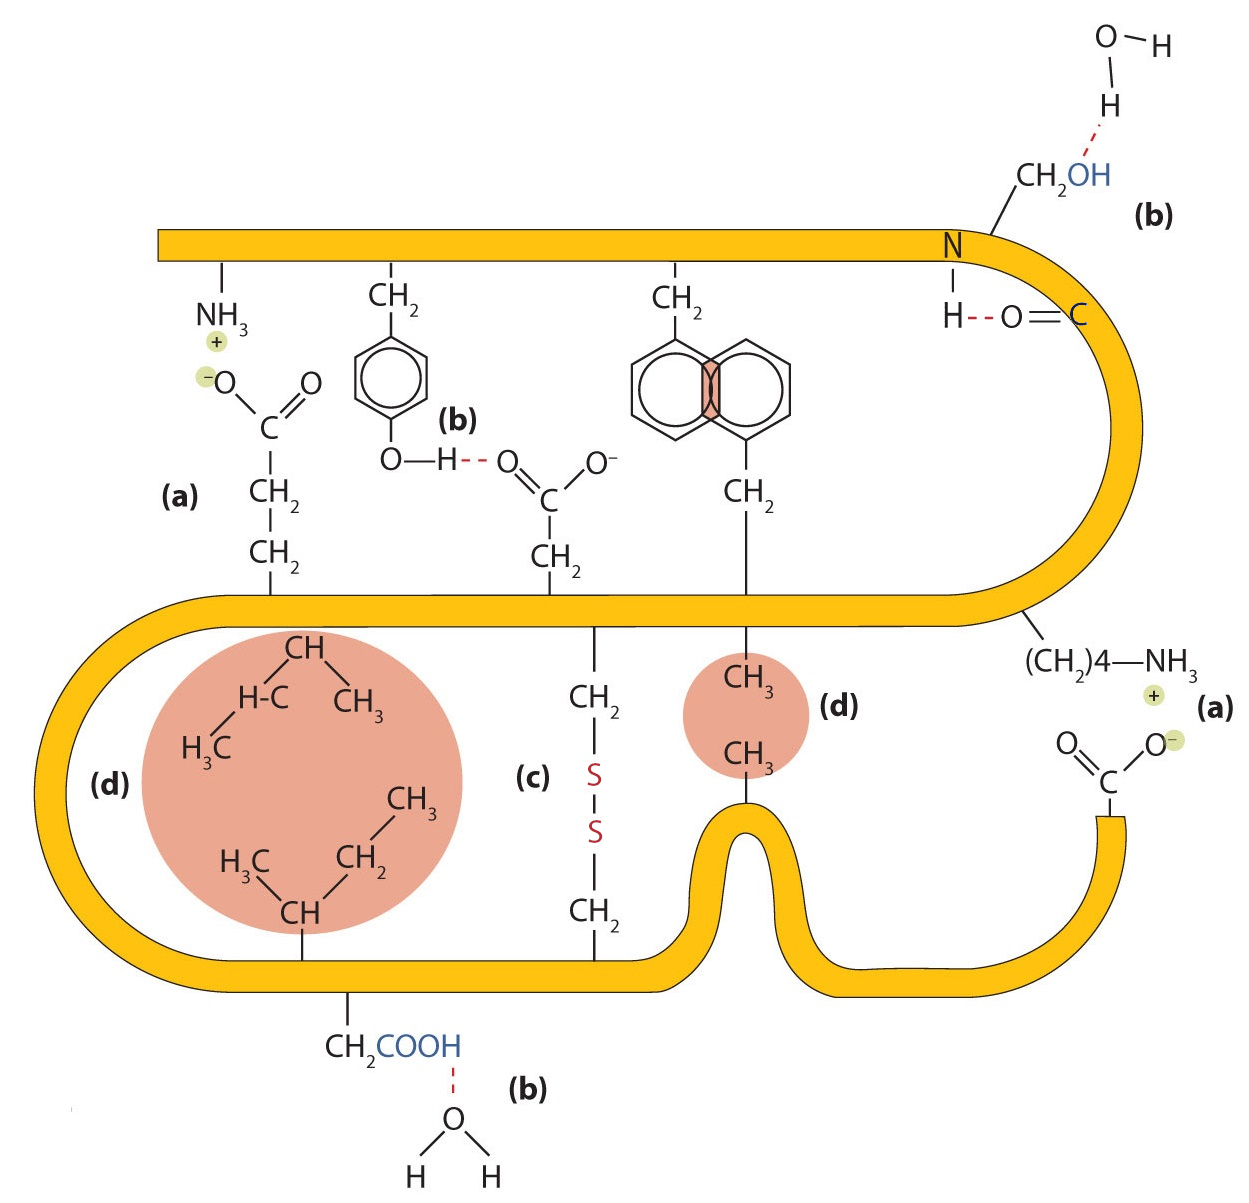
\includegraphics[width = 0.6\textwidth]{figs/interactions-01.png}
\caption{Cuatro interacciones estabilizan la estructura terciaria de una proteína: (a) enlace iónico, (b) enlace de hidrógeno, (c) enlaces disulfuro y (d) fuerzas de dispersión.}
\label{fig:interactions}
\end{figure}

Otras interacciones intramoleculares menos frecuentes podrían ser relevantes en algunas proteínas, como los llamados enlaces isopéptidos, formados entre dos grupos proteicos, al menos uno de los cuales no es un grupo $\alpha$-amino o $\alpha$-carboxi. Algunos ejemplos son la ubiquitilación, la sumoilación, la transglutaminación, el anclaje de proteínas a la superficie celular mediado por sortasas y la formación de pilus. Todos estos procesos comparten varias características (figura \ref{fig:iso}):
\begin{itemize}
\item Todos implican la reacción de un grupo $\epsilon$-amino de la lisina de una proteína con el grupo $\alpha$-carboxi principal de otra proteína, excepto en el caso de la transglutaminación, en la que la lisina se dirige a un grupo carboxiamida de la cadena lateral de la glutamina.
\item Todos los procesos están mediados por enzimas e implican un intermediario tioéster transitorio formado por la cisteína del sitio activo. Este intermediario se resuelve mediante un ataque nucleofílico por el grupo $\epsilon$-amino de la lisina, que completa la formación del enlace.
\end{itemize}

\begin{figure}[h]
\centering
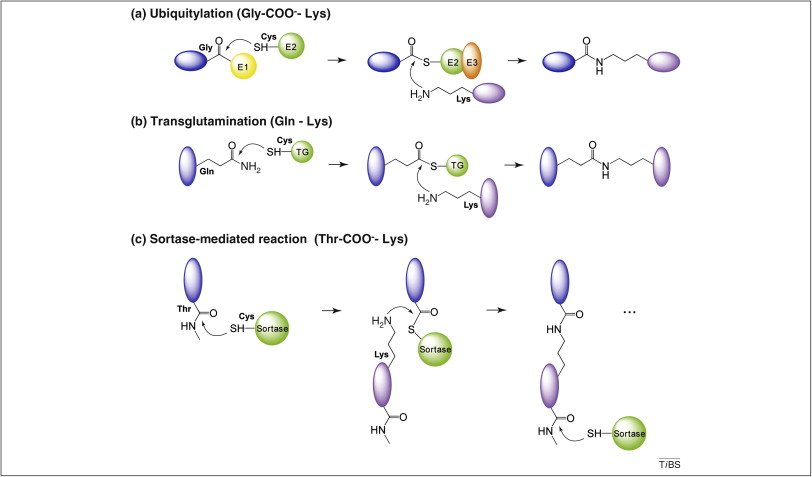
\includegraphics[width = 0.8\textwidth]{figs/iso.jpg}
\caption{Formación de enlaces isopeptídicos intermoleculares mediada por enzimas. Se muestran ejemplos de tres procesos biológicos diferentes: ubiquitilación, transglutaminación y ensamblaje de pilus mediado por sortasa en bacterias Gram positivas. Las proteínas unidas por enlaces isopeptídicos están coloreadas en azul y morado y las enzimas formadoras de enlaces isopeptídicos en verde.}
\label{fig:iso}
\end{figure}

A diferencia de estos procesos dependientes de enzimas, los enlaces isopeptídicos entrecruzados (intrachain isopeptide bonds) se forman autocatalíticamente en la pilina principal Spy0128 de \textit{S. pyogenes} y en otras proteínas de la superficie de células Gram+, así como en la cápside del fago HK97. En este caso, la reacción de formación del enlace es una reacción inducida por la proximidad que se produce cuando los aminoácidos participantes se sitúan juntos en un entorno hidrofóbico, ya sea a través del plegamiento de la proteína concurrente con la formación del enlace peptídico en el ribosoma o por la reorganización de la cápside (en HK97).

En cuanto a la ingeniería proteica, es posible crear aminoácidos no naturales reactivos. Esto se ha utilizado para aumentar la termoestabilidad de proteínas como anticuerpos, crear recombinantes y unir covalentemente proteínas a superficies o nanopartículas.

\subsection{Gráfico de Ramachandran}
Muchas combinaciones de ángulos $\phi$ y $\psi$ están prohibidas debido al principio de exclusión estérica, que dicta que dos átomos no pueden ocupar el mismo espacio simultáneamente. Este concepto fue demostrado inicialmente por Gopalasamudram Ramachandran, que desarrolló un gráfico para visualizar los valores de ángulo permitidos, conocido como gráfico de Ramachandran. Este gráfico puede mostrar los ángulos de un aminoácido específico, de todos los aminoácidos de una proteína o incluso de muchas proteínas. El análisis de los ángulos $\phi$ y $\psi$ en proteínas conocidas revela que aproximadamente tres cuartas partes de todas las combinaciones posibles de $\phi$, $\psi$ no están permitidas (figura \ref{fig:ramachandran}) y se corresponden con motivos comunes de estructura secundaria (figura \ref{fig:ramachandran2}).

\begin{figure}[h]
\centering
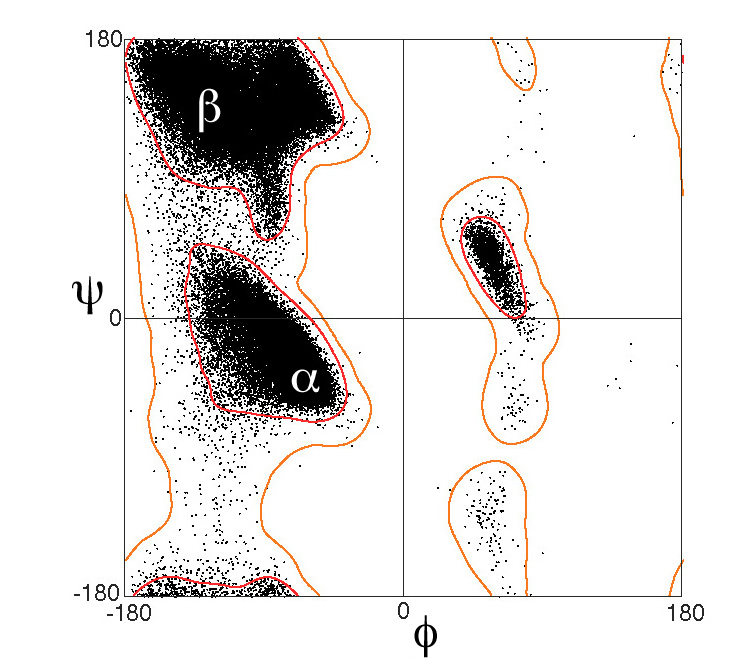
\includegraphics[width = 0.6\textwidth]{figs/Ramachandran_plot_general_100K.jpg}
\caption{Diagrama general de Ramachandran. La densidad de puntos refleja la probabilidad de cada combinación de ángulos, definiendo las regiones central (línea roja) y de tolerancia (naranja).}
\label{fig:ramachandran}
\end{figure}

\begin{figure}[h]
\centering
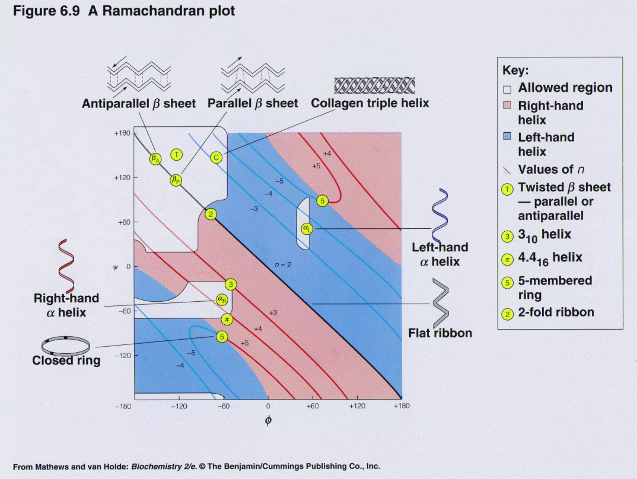
\includegraphics[width = 0.6\textwidth]{figs/rama2.png}
\caption{Definición de alternativas de estructura secundaria por su combinación de ángulos phi, psi.}
\label{fig:ramachandran2}
\end{figure}

Los residuos funcionalmente relevantes son más propensos que otros a tener ángulos de torsión que se sitúan en las regiones permitidas pero desfavorecidas de un diagrama de Ramachandran. La geometría específica de estos residuos relevantes desde el punto de vista funcional, aunque desfavorable desde el punto de vista energético, puede ser importante para la función de la proteína, ya sea catalítica o de otro tipo. Tales conformaciones deben ser estabilizadas por la proteína mediante enlaces H, empaquetamiento estérico u otros medios, y rara vez se dan en residuos muy expuestos a disolventes.

Suele haber espacios designados para las hélices $\alpha$ y las láminas $\beta$, pero también puede haber outliers que muestren aminoácidos concretos.

\subsection{Pliegues (folds), dominios y motivos de proteínas}
La estructura terciaria tridimensional global de una proteína se conoce comúnmente como su \textbf{pliegue}, definiendo así la forma y orientación global ignorando los loops. Dentro del pliegue proteico global, podemos reconocer distintos dominios y motivos. Los \textbf{dominios} son secciones compactas de la proteína que representan regiones estructural y (normalmente) funcionalmente independientes. Eso significa que un dominio mantiene sus características principales, aunque se separe de la proteína global. Por otro lado, los \textbf{motivos} son pequeñas subestructuras que no son necesariamente independientes y que constan sólo de unos pocos tramos de estructura secundaria. De hecho, los motivos también pueden denominarse superestructuras secundarias y son frecuentes en la secuencia. En resumen, un dominio corresponde a un fold, y una cadena peptídica puede tener uno o varios dominios.

La diversidad de pliegues, dominios y motivos proteicos, así como su combinación, puede utilizarse para clasificar jerárquicamente las estructuras proteicas, como en muchos otros campos de la biología. La primera clasificación se propuso en los años 70 y consistía en cuatro grupos de pliegues, como se muestra en la siguiente figura. Todas las proteínas $\alpha$ se basan casi por completo en una estructura $\alpha$-hélice, y todas las estructuras $\beta$ se basan en $\beta$-láminas. La estructura $\alpha$/$\beta$ se basa en una mezcla de $\alpha$-hélices y $\beta$-láminas, a menudo organizadas como $\beta$-hebras paralelas conectadas por $\alpha$-hélices. Por otro lado, las estructuras $\alpha$+$\beta$ consisten en motivos discretos de $\alpha$-hélice y $\beta$-lámina que no están entrelazados (como ocurre en las proteínas $\alpha$/$\beta$). Por último, las proteínas pequeñas abarcan polipéptidos con estructuras secundarias nulas o escasas.

\begin{figure}[h]
\centering
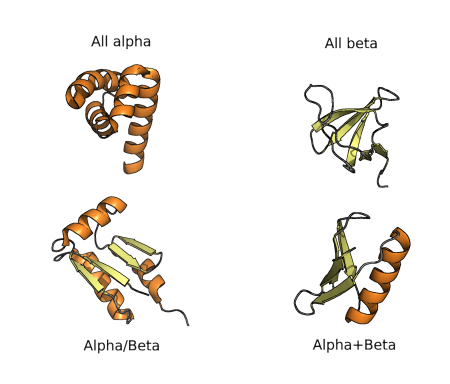
\includegraphics[width = 0.6\textwidth]{figs/clasif.png}
\caption{Las cuatro clases de proteínas estructurales de la clasificación de Chlothia y Levitt.}
\label{fig:alphabeta}
\end{figure}


\end{document}
